\section{Theoretical Analysis}
\label{sec:analysis}


In this section we will detail the theoretical study of the Amplifier Circuit conducted during this lab. The circuit was divided into two seperate ones: the gain stage and the outrput stage. The first one increased the gain, but it had a drop of current considered undesirable due to the output impedance. The latter one corrects this effect while having a gain near one, as to not decrease the voltage previously gained.\\
The entire circuit can be seen in the following image:\\

\FloatBarrier
\begin{document}
\begin{figure}
  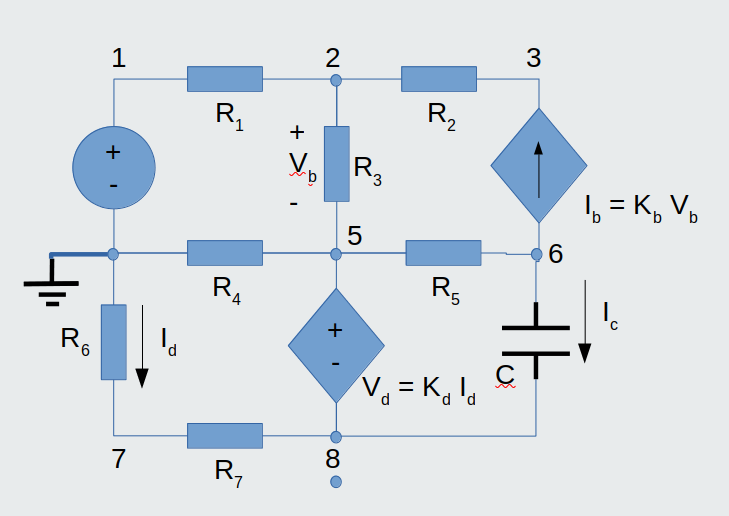
\includegraphics{circuit.ong}
  \caption{}
  \label{}
\end{figure}
\FloatBarrier

One must note that Vin and Rin constitute the thevenin equivalent of the circuit to which the amplifier is connected.\\
The capacitator connected to Rin will enforce that only the AC part of the voltage is taken into account. The DC part is suplied by a constant 12V voltage source Vcc. With this arquitecture, we can ensure that the transistors are in foward active region (FAC), for the Vcc will force an voltage drop bigger than the one necessary for that mode of operation.\\
It was used an Operanting Point analysis where the DC component of the current and voltage is taken into account, but not the AC one, followed by an Incremental Analysis where the AC component of the current and voltage is taken and where a linear model of the transistor is assumed. By adding the results, we can obtain a solution for the circuit, thereby obtaining the values necessary to compute the theoretical gain of the amplifier and the various impedances, such as the input and output ones.
The analysis can be divided into the following particular smaller analysis:
\begin{itemize}
	\item Operating Point analysis for the gain stage;
	\item Incremental analysis for the gain stage;
	\item Calculation of the gain for the gain stage;
	\item Operanting Point analysis for the output stage;
	\item Incremental analysis for the output stage;
	\item Calculation of the gain for the output stage;
	\item Calculation of the input and output inpedances;
\end{itemize}
This analysis was repeated for various frequencies of Vin, and the results were ploted on a dB scale.

%Colocar as equações do slide 6 do power point número 17 - confirmar se o circuito é o mesmo

%Obendo então os seguinte valores explícitos na tabala em baixo

\FloatBarrier
\begin{table}[h]
  \centering
  \begin{tabular}{|c|c|}
    \hline    
    \input{nome do ficheiro}
    \hline
  \end{tabular}
  \caption{Operating point analysis using Octave}
  \label{tab:Octave}
\end{table}
\FloatBarrier    



\par Then, gain, input and output impedances were also obtained for two different states, namely for the gain stage and the output stage.
 The equations used to compute the results for the Gain stage are as follows:

% fórmulas do slide 8 ou 12 de acordo se não tem ou tem o circuito com o bypass C - gain  

\begin{equation}
  \frac{v_o}{v_i} = -g_{m}(\frac{1}{R_C}+\frac{1]{r_o})v_{pi}
  \label{}
\end{equation}   

where: 

\begin{equation}
  v_{pi} = \frac{\frac{1}{r_{pi}}+\frac{1}{R_{B1}}+\frac{1}{R_{B2}}}{R_{S}+(\frac{1}{r_{pi}}+\frac{1}{R_{B1}}+\frac{1}{R_{B2}})}v_{s}
  \label{}
\end{equation}   

%  fórmulas do slide 13  

\begin{equation}
  Z_{I}=\\frac{1}{R_{B1}}+\\frac{1}{R_{B2}}+\frac{1}{r_{pi}}
  \label{}
\end{equation}  

\begin{equation}
  
Z_{O}=\frac{1}{R_{C}}+\frac{1}{R_{o}}}
  \label{}
\end{equation}

\par In parallel, the equations involved in computing for the Output stage are as follows:

% fórmulas do slide 15 - gain  
\begin{equation}
  
\frac{v_{o}}{v_{i}}=\frac{g_m}{g_{pi}+g_{E}+g_{o}+g{m}}
  \label{}
\end{equation}

where g's are the admitances. 

\begin{equation}
  
Z_{I}=\frac{g_{pi}+g_{E}+g_{o}+g{m}}{g_{pi}(g_{pi}+g_{E}+g_{o})}
  \label{}
\end{equation}

\begin{equation}
  
Z_{O}=\frac{1}{g_{pi}+g_{E}+g_{o}+g{m}}
  \label{}
\end{equation}


% fórmulas do slide 16 - impedances 

Using the Octave software, the following values ​​were obtained:

\FloatBarrier
\begin{table}[h]
  \centering
  \begin{tabular}{|c|c|}
    \hline    
    \input{nome do ficheiro}
    \hline
  \end{tabular}
  \caption{Voltage gain, Input and Output Impedances for Gain Stage}
  \label{tab:Octave}
\end{table}
\FloatBarrier    

\FloatBarrier
\begin{table}[h]
  \centering
  \begin{tabular}{|c|c|}
    \hline    
    \input{nome do ficheiro}
    \hline
  \end{tabular}
  \caption{Volatge gain, Input and Output Impedances for Output Stage}
  \label{tab:Octave}
\end{table}
\FloatBarrier     

% Explicar porque é que podem ser ligadas sem ocorrer uma perda significate de sinal

Finally, a study was carried out in the frequency domain for the incremental circuit of voltage gain, then obtaining the graph in dB or SOMETHING LIKE THIS: 


\begin{figure} [!htb] 
  \minipage{0.9\textwidth}
  \includegraphics[width=\linewidth]{nome do ficheiro}
  \caption{Frequency response of Voltage gain in Gain stage}
  \label{fig:theoplots}
  \endminipage\hfill
\end{figure}




